\documentclass{beamer}

\usepackage[italian]{babel}
\usepackage[T1]{fontenc}
\usepackage{beamerthemeAntibes}
\usepackage{graphicx}
\usepackage{listings}
\usepackage[utf8]{inputenc} 
\usepackage{epsfig}  
\usepackage{amsmath} 
\usepackage{multicol}
\usepackage{amsfonts}
\usepackage{hyperref}
\usepackage{listings}

\lstset{
  basicstyle=\footnotesize,
  language=C,                % choose the language of the code                 % where to put the line-numbers
  backgroundcolor=\color{white},  % choose the background color. You must add \usepackage{color}
  showspaces=false,               % show spaces adding particular underscores
  showstringspaces=false,         % underline spaces within strings
  showtabs=true,                 % show tabs within strings adding particular underscores
  tabsize=2,                      % sets default tabsize to 2 spaces
  captionpos=b,                   % sets the caption-position to bottom
  breaklines=true,                % sets automatic line breaking
  breakatwhitespace=true,         % sets if automatic breaks should only happen at whitespace
  title=\lstname,                 % show the filename of files included with \lstinputlisting;
}



\setbeamertemplate{itemize/enumerate body begin}{\footnotesize}

\title{Threshold-Free Cluster Enhancement}
\author{Luigi Giugliano$^1$, Marco Mecchia$^1$}
\institute{$^1$Università degli studi di Salerno}


\begin{document}

\begin{frame}
   \maketitle
\end{frame}

\begin{frame}
  \frametitle{Overview}
  \footnotesize \tableofcontents
\end{frame}

\AtBeginSection[]
  {
     \begin{frame}<beamer>
     \frametitle{Overview}
   \footnotesize \tableofcontents[currentsection]
     \end{frame}
}

\section{Introduzione al problema}

\subsection{Cluster-based thresholding}
\begin{frame}
\frametitle{Spatial information enhancing}
\begin{itemize}

\item Tecnica che prevede l'utilizzo di informazioni spaziali per aumentare l'autenticità di estese aree di segnale. 
\vfill
\item La motivazione risiede nel fatto che le regioni del segnale sono più estese del rumore e quindi trovare zone aumenta la possibilità che esse siano segnale vero e proprio e non rumore.
\end{itemize}

\end{frame}

\begin{frame}
\frametitle{Cluster-based Thresholding}
\begin{itemize}
\item L'approccio pi\'u comune in neuroimaging.
\vfill
\item Problemi:
\begin{itemize}
\item Necessit\'a di definire una soglia di clustering.
\item Sogliatura di tipo \emph{hard}
\item Difficolt\'a nel riconoscimento di eventuali \emph{subcluster}
\end{itemize}
\end{itemize}
\end{frame}

\subsection{Threshold Free Cluster Enhanchment}

\begin{frame}
\frametitle{Overview dell'algoritmo}
\begin{itemize}
\item Procedura che tenta di superare i problemi degli approcci precedenti.
\item Input: Un immagine statistica non processata.
\item Output: Un immagine statistica in cui il valore di ogni voxel \'e un \alert{punteggio} che rappresenta il contributo spaziale del cluster di cui fa parte.
\end{itemize}
\vfill
\begin{itemize}
\item Clustering dell'immagine \alert{intrinseco}.
\end{itemize}
\end{frame}

\begin{frame}
\frametitle{Assegnazione dei punteggi(1/2)}
Il punteggio del voxel $p$ viene stabilito dalla seguente formula:

$$TFCE(p)=\int_{h=h_0}^{h_p}e(h)^E h^H dh$$
dove:
\begin{itemize}
\item $h_p$ \'e il punteggio statistico del voxel $p$.
\item $e(h)$ \'e l'area del cluster ad altezza $h$.
\item $E$ ed $H$ sono costanti.
\end{itemize}
\vfill
Questo integrale viene calcolato in pratica tramite una sommatoria ponendo $dh = 0.1$.

\end{frame}

\begin{frame}
\frametitle{Assegnazione dei punteggi(2/2)}
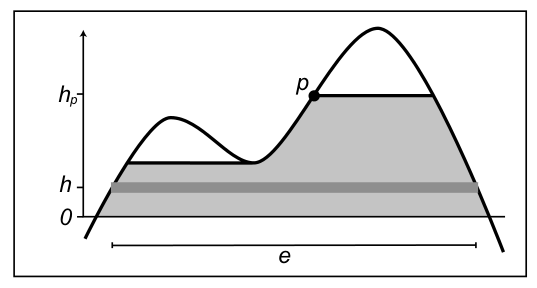
\includegraphics[width=300px]{Images/TFCE.png}
\end{frame}

\section{Codice}
\subsection{Suddivisione del codice}
\begin{frame}
\frametitle{Suddivisione del codice}
I file principali che compongono il plugin sono:
\begin{itemize}
\item{Tfce.cpp}
\item{Utilities.cpp}
\end{itemize}
\vfill
\textbf{Tfce} è il core del plugin, dove avviene il  calcolo dei punteggi.\\
\smallskip
\textbf{Utilities} contiene tutte le funzioni di supporto.
\end{frame}

\begin{frame}[fragile]
\frametitle{Funzioni pubbliche (1/3)}
L' unica funzione che viene esposta dal file \textbf{Tfce.h} è:
\begin{center}
\begin{lstlisting}
float * tfce_score(float * map, int dim_x, int dim_y, int dim_z, float E, float H, float dh);
\end{lstlisting}
\end{center}
\end{frame}

\begin{frame}[fragile]
\frametitle{Funzioni pubbliche (2/3)}
Le funzioni che espone \textbf{Utilities.h} sono:
\begin{center}
\begin{lstlisting}
void findMinMax(float *map, int n, float *min, float *max, float * range);

int confront(float a, float b, char operation);

int * getBinaryVector(float * map, int n, int (*confront)(float, float), float value, int *      numOfElementsMatching);
\end{lstlisting}
\end{center}
\end{frame}

\begin{frame}[fragile]
\frametitle{Funzioni pubbliche (3/3)}
\begin{center}
\begin{lstlisting}
float * fromBinaryToRealVector(float * map, int n, int * binaryVector);

float * fill0(int n);

void apply_function(float * vector, int n, float (* operation) (float a, float b), float argument);

int linearIndexFromCoordinate(int x, int y, int z, int max_x, int max_y);

void coordinatesFromLinearIndex(int index, int max_x, int max_y, int * x, int * y, int * z);

float * copyAndConvertIntVector(int * vector, int n);
\end{lstlisting}
\end{center}
\end{frame}

\subsection{Dettagli implementativi}
\begin{frame}[fragile]
\frametitle{Dettagli della funzione tfce score}
\begin{center}
\begin{lstlisting}
float * tfce_score(float * map, int dim_x, int dim_y, int dim_z, float E, float H, float dh){
	findMinMax(map, n, &minData, &maxData, &rangeData);
	precision = rangeData/dh;
	if (precision > 200) {
		increment = rangeData/200;
	} else{
		increment = rangeData/precision;	
	}
	steps = ceil((maxData - minData) / (increment));
	#pragma omp parallel for
	for (i = 0; i < steps; i++) {
		 computeTfceIteration(minData + i*increment, map, n, dim_x, dim_y, dim_z, E, H, dh, toReturn);
	}	
	return toReturn;
}
\end{lstlisting}
\end{center}
\end{frame}

\begin{frame}[fragile]
Funzione \textbf{computeTfceIteration}:
\begin{center}
\begin{lstlisting}
int * indexMatchingData = getBinaryVector(map, n, moreThan, h, &numOfElementsMatching);
clustered_map = find_clusters_3D(indexMatchingData, dim_x, dim_y, dim_z, n, &num_clusters);
extent_map = new int[n];
for (j = 0; j < n; ++j){
    extent_map[j] = 0;
}
delete [] indexMatchingData;
for (i = 1; i <= num_clusters; ++i) {
    numOfElementsMatching = 0;	
    for (j = 0; j < n; ++j){
        if(clustered_map[j] == i){
            numOfElementsMatching++; }}
    for (j = 0; j < n; ++j) {
       if(clustered_map[j] == i)
           extent_map[j] = numOfElementsMatching; }}
\end{lstlisting}
\end{center}
\end{frame}

\begin{frame}[fragile]
\begin{center}
\begin{lstlisting}
clustered_map_float = copyAndConvertIntVector(extent_map, n);
apply_function(clustered_map_float, n, elevate, E);
apply_function(clustered_map_float, n, multiply, pow(h, H));
apply_function(clustered_map_float, n, multiply, dh);
for (i = 0; i < n; ++i) {
#pragma omp atomic
    toReturn[i] += (clustered_map_float[i]);
}
delete[] clustered_map_float;
delete[] clustered_map;
delete[] extent_map;
\end{lstlisting}
\end{center}
\end{frame}

\begin{frame}[fragile]
Funzione \textbf{getBinaryVector}:
\begin{center}
\begin{lstlisting}
int * getBinaryVector(float * map, int n, int (*confront)(float, float), float value, int * numOfElementsMatching){
    int * binaryVector = new int [n];
    (*numOfElementsMatching) = 0;
    int i;
    for (i = 0; i < n; ++i) {
        if(confront(map[i],value)){
            binaryVector[i] = 1;
            (*numOfElementsMatching)++;
        }
        else
            binaryVector[i] = 0;
        }
    return binaryVector;
}
\end{lstlisting}
\end{center}
\end{frame}

\begin{frame}[fragile]
\frametitle{Find connected components in binary images (1/2)}
La funzione \textbf{find\_cluster\_3D}:\\
\begin{lstlisting}
int * find_clusters_3D(int * binaryVector, int dim_x, int dim_y, int dim_z, int n, int * num_clusters)
\end{lstlisting}

restituisce la mappa dei cluster trovati utilizzando la \textbf{26-connectivity} nell'immagine binaria fornita in input.
\end{frame}

\begin{frame}
\frametitle{Find connected components in binary images (2/2)}
.
\vfill
\[
\begin{bmatrix}
    1       & 1 & 0 & 1 & 1\\
    1       & 1 & 0 & 0 & 0 \\
    1       & 0 & 1 & 1 & 1 \\
    1       & 0 & 0 & 1 & 1
\end{bmatrix}
=
\begin{bmatrix}
    1       & 1 & 0 & 3 & 3\\
    1       & 1 & 0 & 0 & 0 \\
    1       & 0 & 2 & 2 & 2 \\
    1       & 0 & 0 & 2 & 2
\end{bmatrix}
\]
\end{frame}

\begin{frame}[fragile]
E' stato utilizzata la specifica OpenMP per rendere il calcolo degli score più veloce.\\
\medskip
OpenMP (Open Multiprocessing) è un API multipiattaforma per la creazione di applicazioni parallele su sistemi a memoria condivisa.\\
\smallskip
Il comando:\\
\textbf{\#pragma omp parallel for}\\
viene utilizzato per rendere un for parallelo.\\
\smallskip
Il comando:\\
\textbf{\#pragma omp atomic}\\
invece viene utilizzato per rendere un istruzione atomica.\\
\end{frame}

\begin{frame}
Abbiamo deciso di utilizzare, OMP perché l'effort per utilizzarlo è praticamente nullo, e le prestazioni sono ottime.\\
\medskip
Inoltre essendo che l'implementazione dei \textit{Thread} in \textit{C} cambia tra Windows e Linux, si sarebbe reso necessario modificare il codice per renderlo funzionante su entrambe le piattaforme.
\end{frame}

\end{document}
